\documentclass[a4paper, 12pt]{article}
\usepackage{parskip}   % for formatting paragraphs nicer
\usepackage{graphicx}  % for images
\usepackage{color}
\usepackage{amsmath}   % for text in maths

\makeatletter
\def\@seccntformat#1{%
  \expandafter\ifx\csname c@#1\endcsname\c@section\else
  \csname the#1\endcsname\quad
  \fi}
\makeatother

\title{Physics Notes}
\date{}
\begin{document}

\maketitle

\section{Particles}

\subsection{Classification}

There are two main groups of particles: Hadrons and Leptons.

Hadrons feel the strong force and are made up of quarks. The proton is the only stable baryon, while a neutron left on it's own will decay with a half life of about 11 minutes.

Leptons are fundamental particles like quarks, and do not feel the strong force. They mostly interact through the weak interaction (or EM if charged, and gravitational force as they have mass).
Leptons have a lepton number that is always conserved in a interaction. Neutrinos are leptons and have no charge, and very little mass, so they are hard to detect.

Hadrons consist of two separate families of particles: Baryons and Mesons.

Baryons consist of 3 quarks of any type. Mesons are a quark - anti quark pair.

\begin{center}
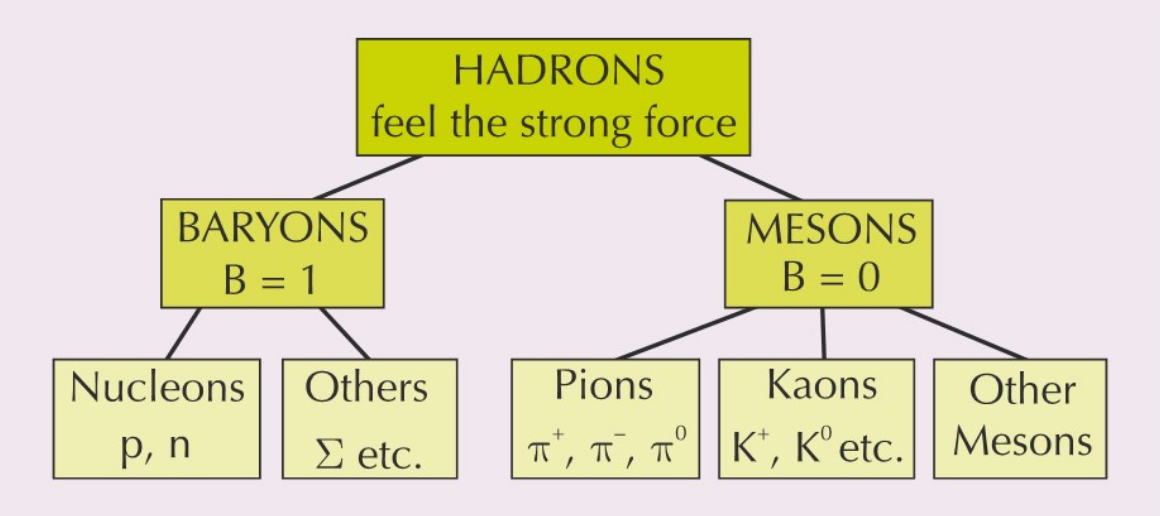
\includegraphics[height=5cm]{hadronFamily.png}
\end{center}

\subsection{Quarks}

Quarks are fundamental particles that make up hadrons.

The only three quarks that you need to know for A-Level is the up quark ($u$), down quark ($d$) and the strange quark ($s$).

Here is the table from the formula sheet showing the properties:

\begin{center}
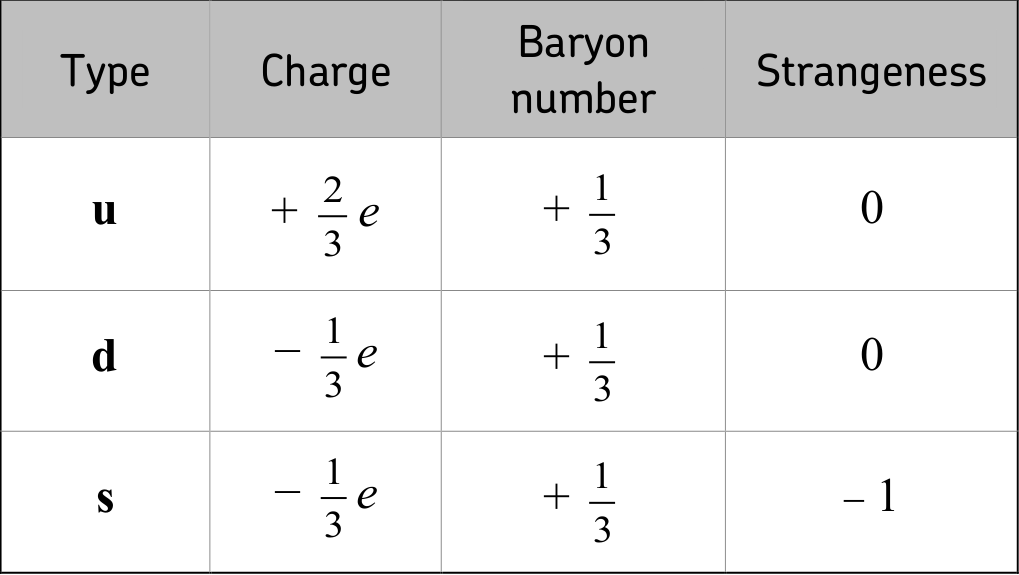
\includegraphics[height=5cm]{quarks.png}
\end{center}

\subsubsection{Conservation Laws}

Conserved in all interactions:
\begin{itemize}
	\item{Baryon number}
	\item{Lepton number}
	\item{Momentum}
	\item{Charge}
\end{itemize}

Strangeness is conserved almost all interactions \colorbox{yellow}{unless it is the weak interaction}, as the weak interaction involves changing the type of a quark.

\subsubsection{Specific Mass}

Specific mass $= \frac{mass}{charge}$

\subsection{Forces}

\subsubsection{Strong Force}

The strong force binds all the nucleons in the nucleus together. It only works between hadrons.

The strong force is {\textbf{repulsive}} at distances $< 0.5$ fm, and {\textbf{attractive}} at distances $> 0.5$ fm to $3$ fm.

The strong force in the nucleus has to be stronger overall (hence the name) than the EM force to keep the nucleus together, as the protons in the nucleus are all repelling each other proton in the nucleus, where as the strong force is much more attractive for the nucleons around it, but has pretty much no effect on other nucleons.

The exchange particle for the strong force is the $\pi$ pion (a meson). (it is actually gluons but we have to say pions).


\subsubsection{Electromagnetic Force}

The electromagnetic force acts between charged particles, where $F \propto \frac{1}{r^2}$, (inverse square law) where $r$ is the distance between the centre's of the particles.

The exchange particle for the EM force is the (virtual) photon ($\gamma$), which has no mass, and travels at the speed of light ($\approx 3 \times 10^8$). It has wave-particle duality.

\subsubsection{Weak Force}

The weak force can act between any two particles. The weak force changes the flavour of a quark. This means that a strange quark can be changed into any other quark, so strangeness may not be conserved in weak interactions. It's pretty weak.

The exchange particle for the weak force is the $W^+$ or $W^-$ boson.

\subsubsection{Gravitational Force}

The gravitational force acts between all particles with mass. Like the EM force, it follows an inverse square law: $F \propto \frac{1}{r^2}$

\subsection{Decays}

Here is a graph showing the different isotopes for varying numbers of neutrons and protons, and what decay is likely to happen to each (unless stable):

\begin{center}
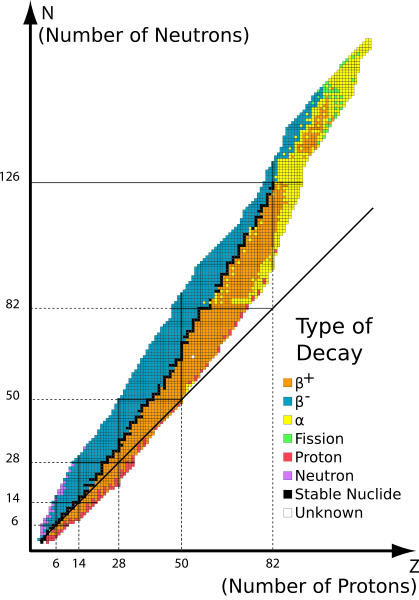
\includegraphics[height=12cm]{bandOfStability.png}
\end{center}

At lead ($Pb\, ^{208}_{82}$), 126 neutrons and 82 protons, the stability line ends.

Neon ($Ne\, ^{20}_{10}$) is the last isotope that follows the projection line exactly.

\subsubsection{{$\alpha$} decay}

Alpha decay is the emission of a helium nucleus from an atom's nucleus.

${\alpha^4_2}$

Alpha decay usually happens in very heavy isotopes that need to get rid of both neutrons and protons, due to the EM force in the nucleus overcoming the strong force between nucleons.

An example alpha decay would be:

$Pu^{\,240}_{\,94}\, {\Rightarrow}\, U^{\,236}_{\,92} + \alpha^4_2$

\subsubsection{{$\beta$} decay}

\textbf{$\beta^-$ decay:}

$\beta^-$ decay is when a neutron turns into a proton and electron via the weak interaction. The exchange particle is $W^-$, easy to remember since it is also negative.

Here is the equation for $\beta^-$ decay:

$n^0_1 \, \rightarrow \, p^+_1 + e^- + \overline{V_e}$

The anti neutrino $\overline{V_e}$ is to balance the lepton 

Here is the feynman diagram for $\beta^-$ decay:

\begin{center}
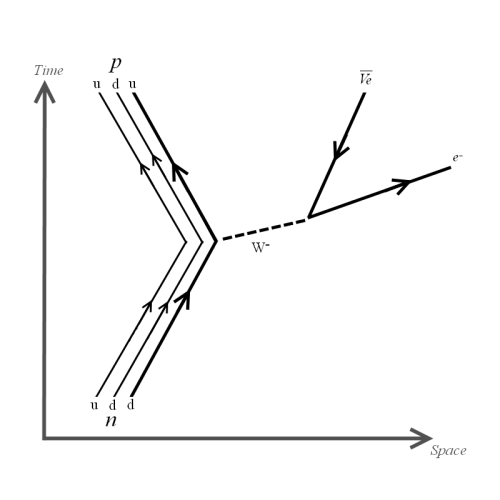
\includegraphics[height=8cm]{betaMinus.png}
\end{center}

\textbf{$\beta^+$ decay:}

$\beta^+$ decay is when a proton turns into a neutron and positron. This is key, as the position will annihilate pretty quickly with a nearby electron (as they are antiparticles), producing two high energy photons (probably gamma), so light will be emitted. The exchange particle this time is a $W^+$ boson.

Here is the equation for $\beta^+$ decay:

$p^+_1 \, \rightarrow \, n^0_1 + e^+ + V_e$

Here is the feynman diagram for $\beta^+$ decay:

\begin{center}
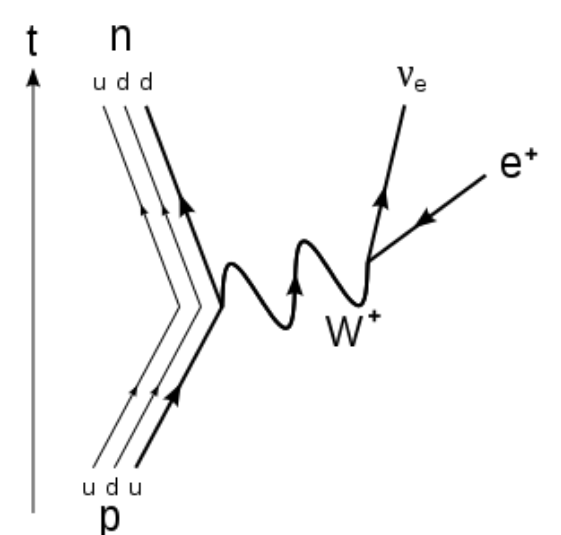
\includegraphics[height=7cm]{betaPlus.png}
\end{center}

It is pretty much the reverse of $\beta^-$.

\subsection{Electron Energy Levels}

Electrons around the nucleus can have different energy levels depending on how far away they are from the nucleus (potential energy). The further away they are from the nucleus, the less energy is required to remove the electron from that energy level and onto a higher one.

\subsection{Pair Production}

If a photon interacts with a nucleus, the energy of the photon can be converted into an electron-positron pair ($energy \rightarrow mass$). This is so that lepton number is conserved.

Here is a diagram:

\begin{center}
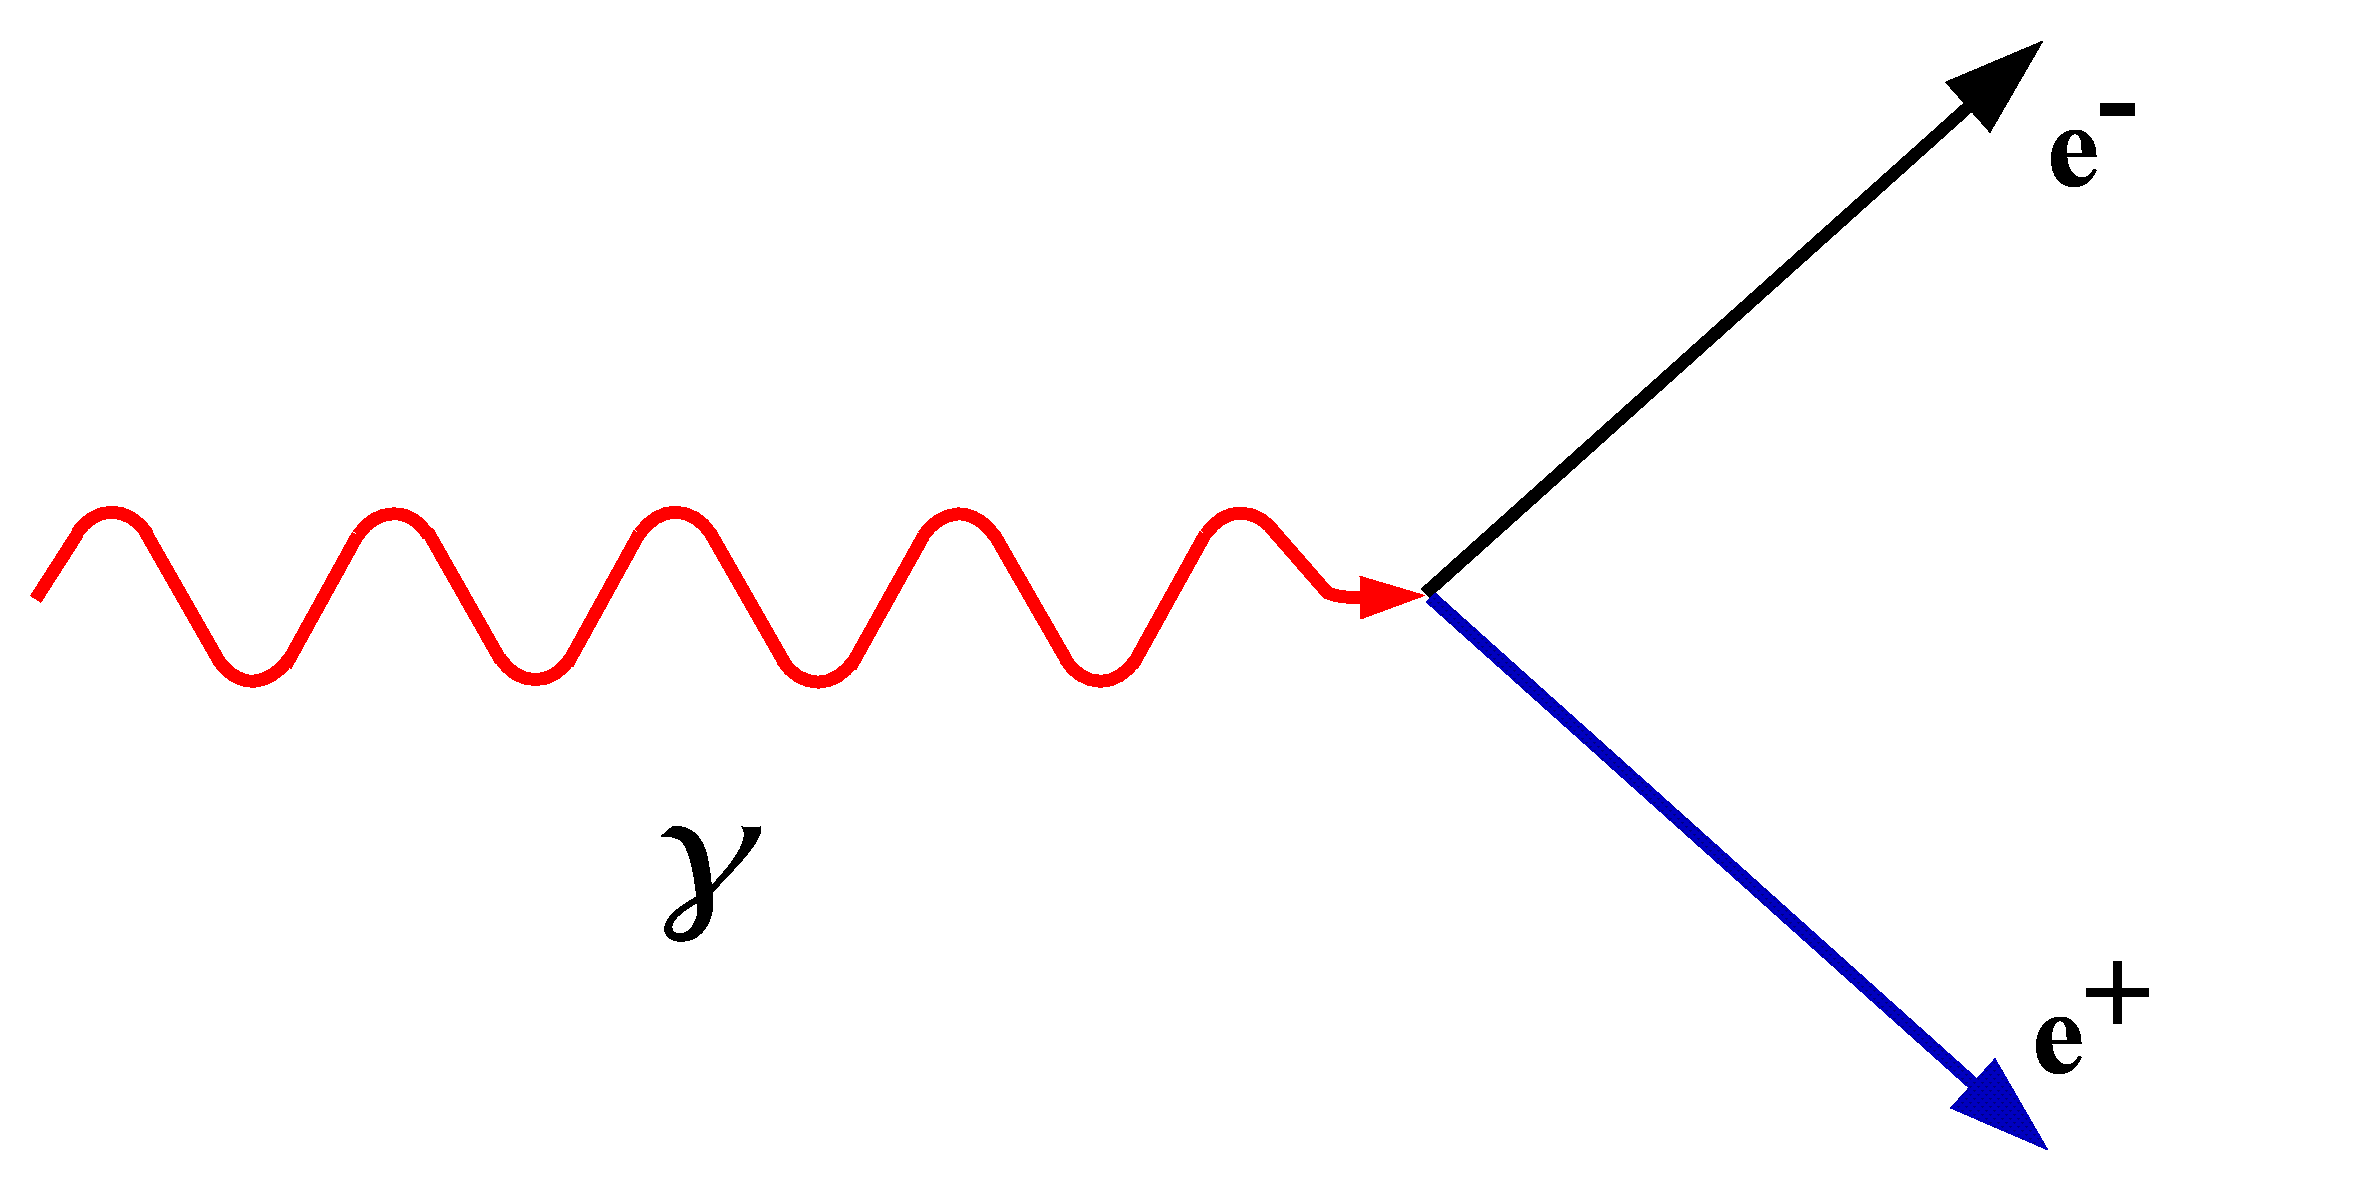
\includegraphics[height=4cm]{pairProduction.png}
\end{center}

\subsection{Electron Capture}

Electron capture is when an electron from one of the electron shells is succed into the nucleus, and interacts with a proton in the nucleus to produce a neutron and an electron neutrino. This is pretty much $\beta^+$, but there is no need for a positron since the electron at the start counteracts the charge of the proton at the start, so charge is 0 on both sides.

The equation is:

$p^+_1 + e^-_0 \, \rightarrow \, n^0_1 + Ve^0_0$

\textbf{It is important to remember that a photon will be released when the electron drops down to the ground state.}

\subsection{EM Repulsion}

When two like-charged particles get close, they repel through the EM force. \textbf{Virtual} photons are exchanged during the interaction:

\begin{center}
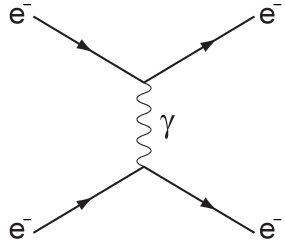
\includegraphics[height=4cm]{emRepulsion.png}
\end{center}

\subsection{Antimatter}

Antiparticles have the same attributes as their regular counterparts, but usually the opposite of everything (including charge).

When two antiparticles collide/interact, they annihilate each other, converting the mass of both of the particles into energy in the form of two photons. \colorbox{yellow}{Two photons are produced to conserve momentum.}

Since antiparticles have opposite charges to their normal counterparts, so annihilation is likely to happen if an antiparticle is nearby. Hence why there is so little antimatter compared to matter, but we do not know why there is overall more regular matter than antimatter.
\newpage

\subsection{The Photoelectric Effect}

The photoelectric effect is the process by which a metal with photons incident on it emits electrons (photoelectrons).

The photon interacts with an electron in the metal, and if the photon has enough energy to liberate the electron, then the electron will be liberated. This minimum energy is the work function ($\phi$).

The work function is the minimum energy required to liberate an electron from the \textit{surface} of the material. Electrons from deeper down in the material require more energy to liberate.

The threshold frequency is the frequency of the photon needed to meet that minimum energy requirement (the work function). The equation for the threshold frequency is:
$$
f = \frac{\phi}{h}
$$

Where $\phi$ is the work function of the material, and $h$ is the planck constant.

The equation you get in the equation sheet is:
$$
hf = \phi + E_{k \, (\text{max})}
$$

The photoelectric effect can be demonstrated using a UV lamp and a charged zinc plate and some gold leaf foil:

\begin{center}
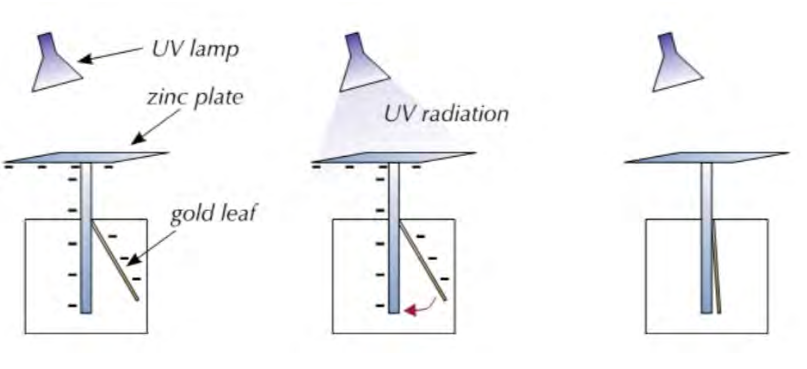
\includegraphics[width=\textwidth]{photoelecExp.png}
\end{center}

\newpage
\subsection{Electron Energy Levels}

Around an atom's nucleus there are discrete energy levels.

\textbf{Excitation} is where an electron bound to an atom moves up one or more energy levels. \textbf{De-excitation} is the opposite. Excitation requires energy to move the electron to a higher state, while de-excitation releases energy in the form of a photon.

\textbf{Ionisation} is where the electron is completely removed from the atom.

\subsubsection{Absorption and Emission lines}

The photons absorbed during excitation, or the photons released during de-excitation can be used to figure out what element the substance is made from, as every atom has different energies required to excite/de-excite electrons.

You can make an emission/absorption spectra to find the emission/absorption lines:

\begin{center}
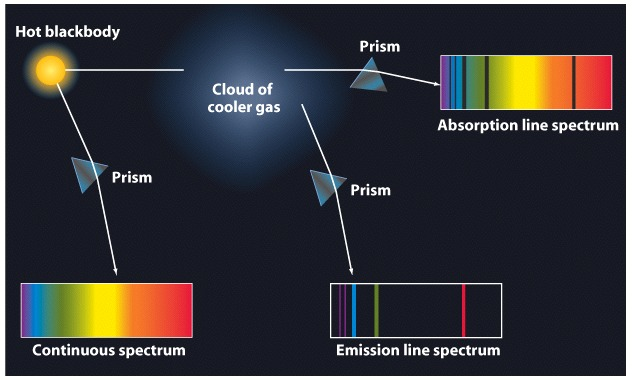
\includegraphics[width=\textwidth]{spectraElecEmmision.jpg}
\end{center}

\subsubsection{Fluorescent Tubes}

Fluorescent tubes work by firing a beam of free electrons from one end to the other.
The tube is filled with mercury gas, so these free electrons collide with electrons in the atoms in the mercury gas, exciting the electrons. The electrons then de-excite releasing UV photons. There is a phosphorus coating on the inside of the tube, and the UV ray excites electrons in the phosphorus, and quickly de-excites to a lower energy level again, which then releases light in the visible spectrum.

Here is an image of the tube:

\begin{center}
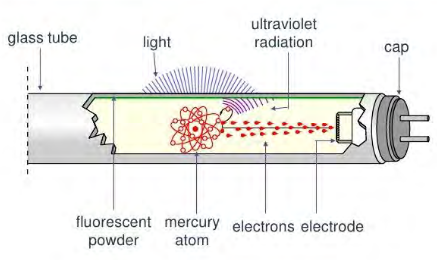
\includegraphics[width=\textwidth]{mercuryTube.png}
\end{center}

\subsection{Wave Particle Duality}

Wave particle duality is when a particle has wave-like properties, as well as particle-like qualities. For example, a photon was always thought to be a wave, however the photoelectric effect disproves this, as it requires light to be discrete packets of energy, rather than just a wave.

Another example of wave particle duality would be that electrons can be diffracted if going through a gap of similar size to the De-Broglie wavelength. However, electrons are clearly particles as they are deflected by electric fields, which shows it is also a particle.

Here is the equation for the De-Broglie wavelength:

$$
\lambda = \frac{h}{p} = \frac{h}{mv}
$$

\newpage
\section{Waves}


\end{document}
